\hypertarget{introduction}{%
\section{Introduction}\label{introduction}}

\newpage

\hypertarget{requirements}{%
\section{Requirements}\label{requirements}}

\newpage

\hypertarget{design-process}{%
\section{Design Process}\label{design-process}}

In order to be able to complete the project to both a high standard an
within a timely manner, a design process was following both process and
agile design methods to reach the projects objectives. The project was
spilt into three phases: \emph{definition, design} and
\emph{development}. Figure \ref{designprocess}, shows an overview of the
projects workflows and a breakdown of the key steps of each phase.

\begin{figure}[H]
\centering
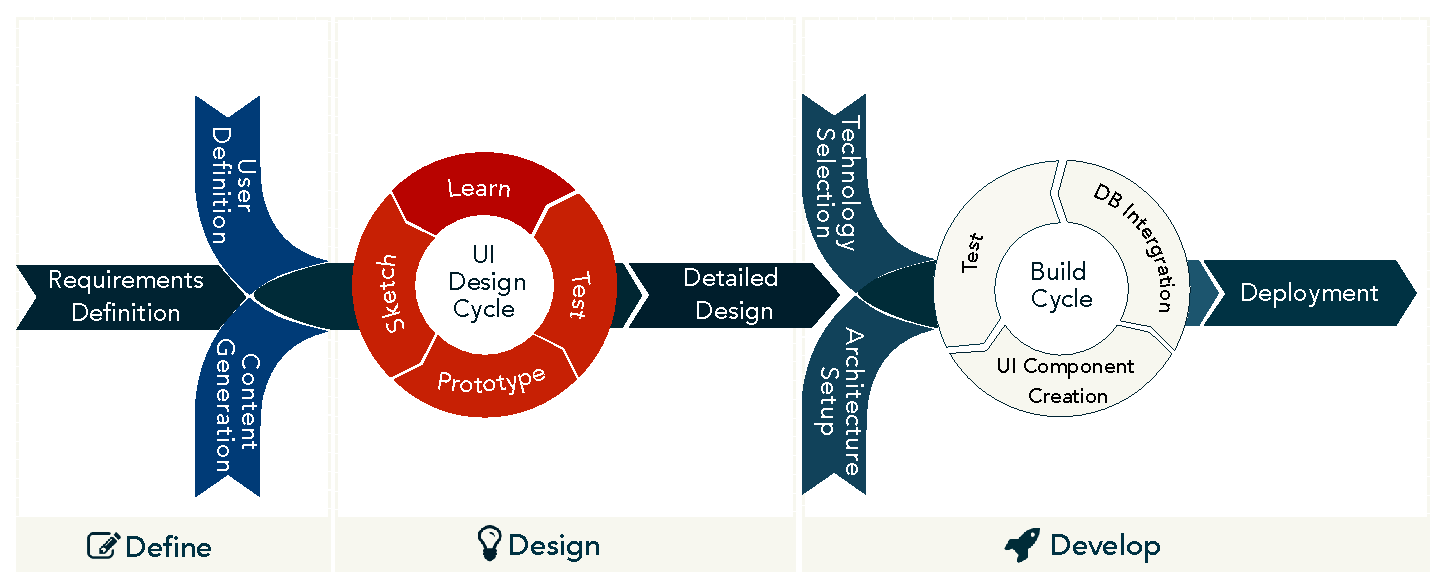
\includegraphics[trim = 0 0 0 0, clip, width=0.98\textwidth]{DesignProcess.eps}
\caption{Diagram illustrating the design process progressing the from the initial briefing to implementation}
\label{designprocess}
\end{figure}

\hypertarget{definition-phase}{%
\subsection{Definition Phase:}\label{definition-phase}}

This phase focused on collecting requirements and defining the
objectives of the project. In order to capture all the information
correctly, several meetings were held with the client these meetings
meetings were used to capture the main features of the site, creating
and organising the content that would be displayed. User research was
then embarked, refining the objectives and content of the site. These
stages all worked towards providing all the prior research required to
begin designing, prototyping and envisioning how the website would
function.

\hypertarget{design-phase}{%
\subsection{Design Phase:}\label{design-phase}}

The design phase applied human computer interaction (HCI) principles in
an agile to approach, to mock up variety of different solutions and
refine the solutions quickly. By following of the process of creating
sketches of different components of the website, whittling these
sketches down to wireframes and prototypes. Solutions could be quickly
tested by the designers, client and user groups providing feedback to
take back and learn upon, improving the overall design of the website
until a rough solution was generated which met both the design
objectives and the met HCI objectives. Spending time before writing any
code was key to making sure the solution was user friendly and visual
meeting one of the key objectives of the project. After rough solution
was created through user interface (UI) design cycle, this was then
padded out and refined creating a static draft of the design which could
be directly copied in the development phase. A large amount of time
could be saved in the development phase of the project by having a
finalised design template to work of which included the typography,
components and the page layouts of the site.

\hypertarget{development-phase}{%
\subsection{Development Phase:}\label{development-phase}}

Development was the final phase of the project. A complete understanding
of how the final product will look and function, based on the research
conducted in the definition phase and the detailed design template in
the design phase meant that all the technology required to required to
implement the solution can be selected. A local development environment
shared amongst all the developers enabled the use of an agile build
cycle, using git to mediate between the different versions. The build
cycle consisted of a developer taking a UI component from the template
and creating the design in code. This would then be connected to the PHP
database using word-press and the tested. Any bugs in either the design
or functionality could then be ironed out through iteration through the
cycle eventually integrating all the components together into the final
site. Once the entire design template was implemented the project could
then be deployed onto the web.

\newpage

\hypertarget{user-research}{%
\section{User Research}\label{user-research}}

this is some nice text bellow is an image.
\cite{blanchard2003macroeconomic}

\hypertarget{this-is-a-sub-heading}{%
\subsection{This is a sub heading}\label{this-is-a-sub-heading}}

\begin{figure}[H]
      \centering
      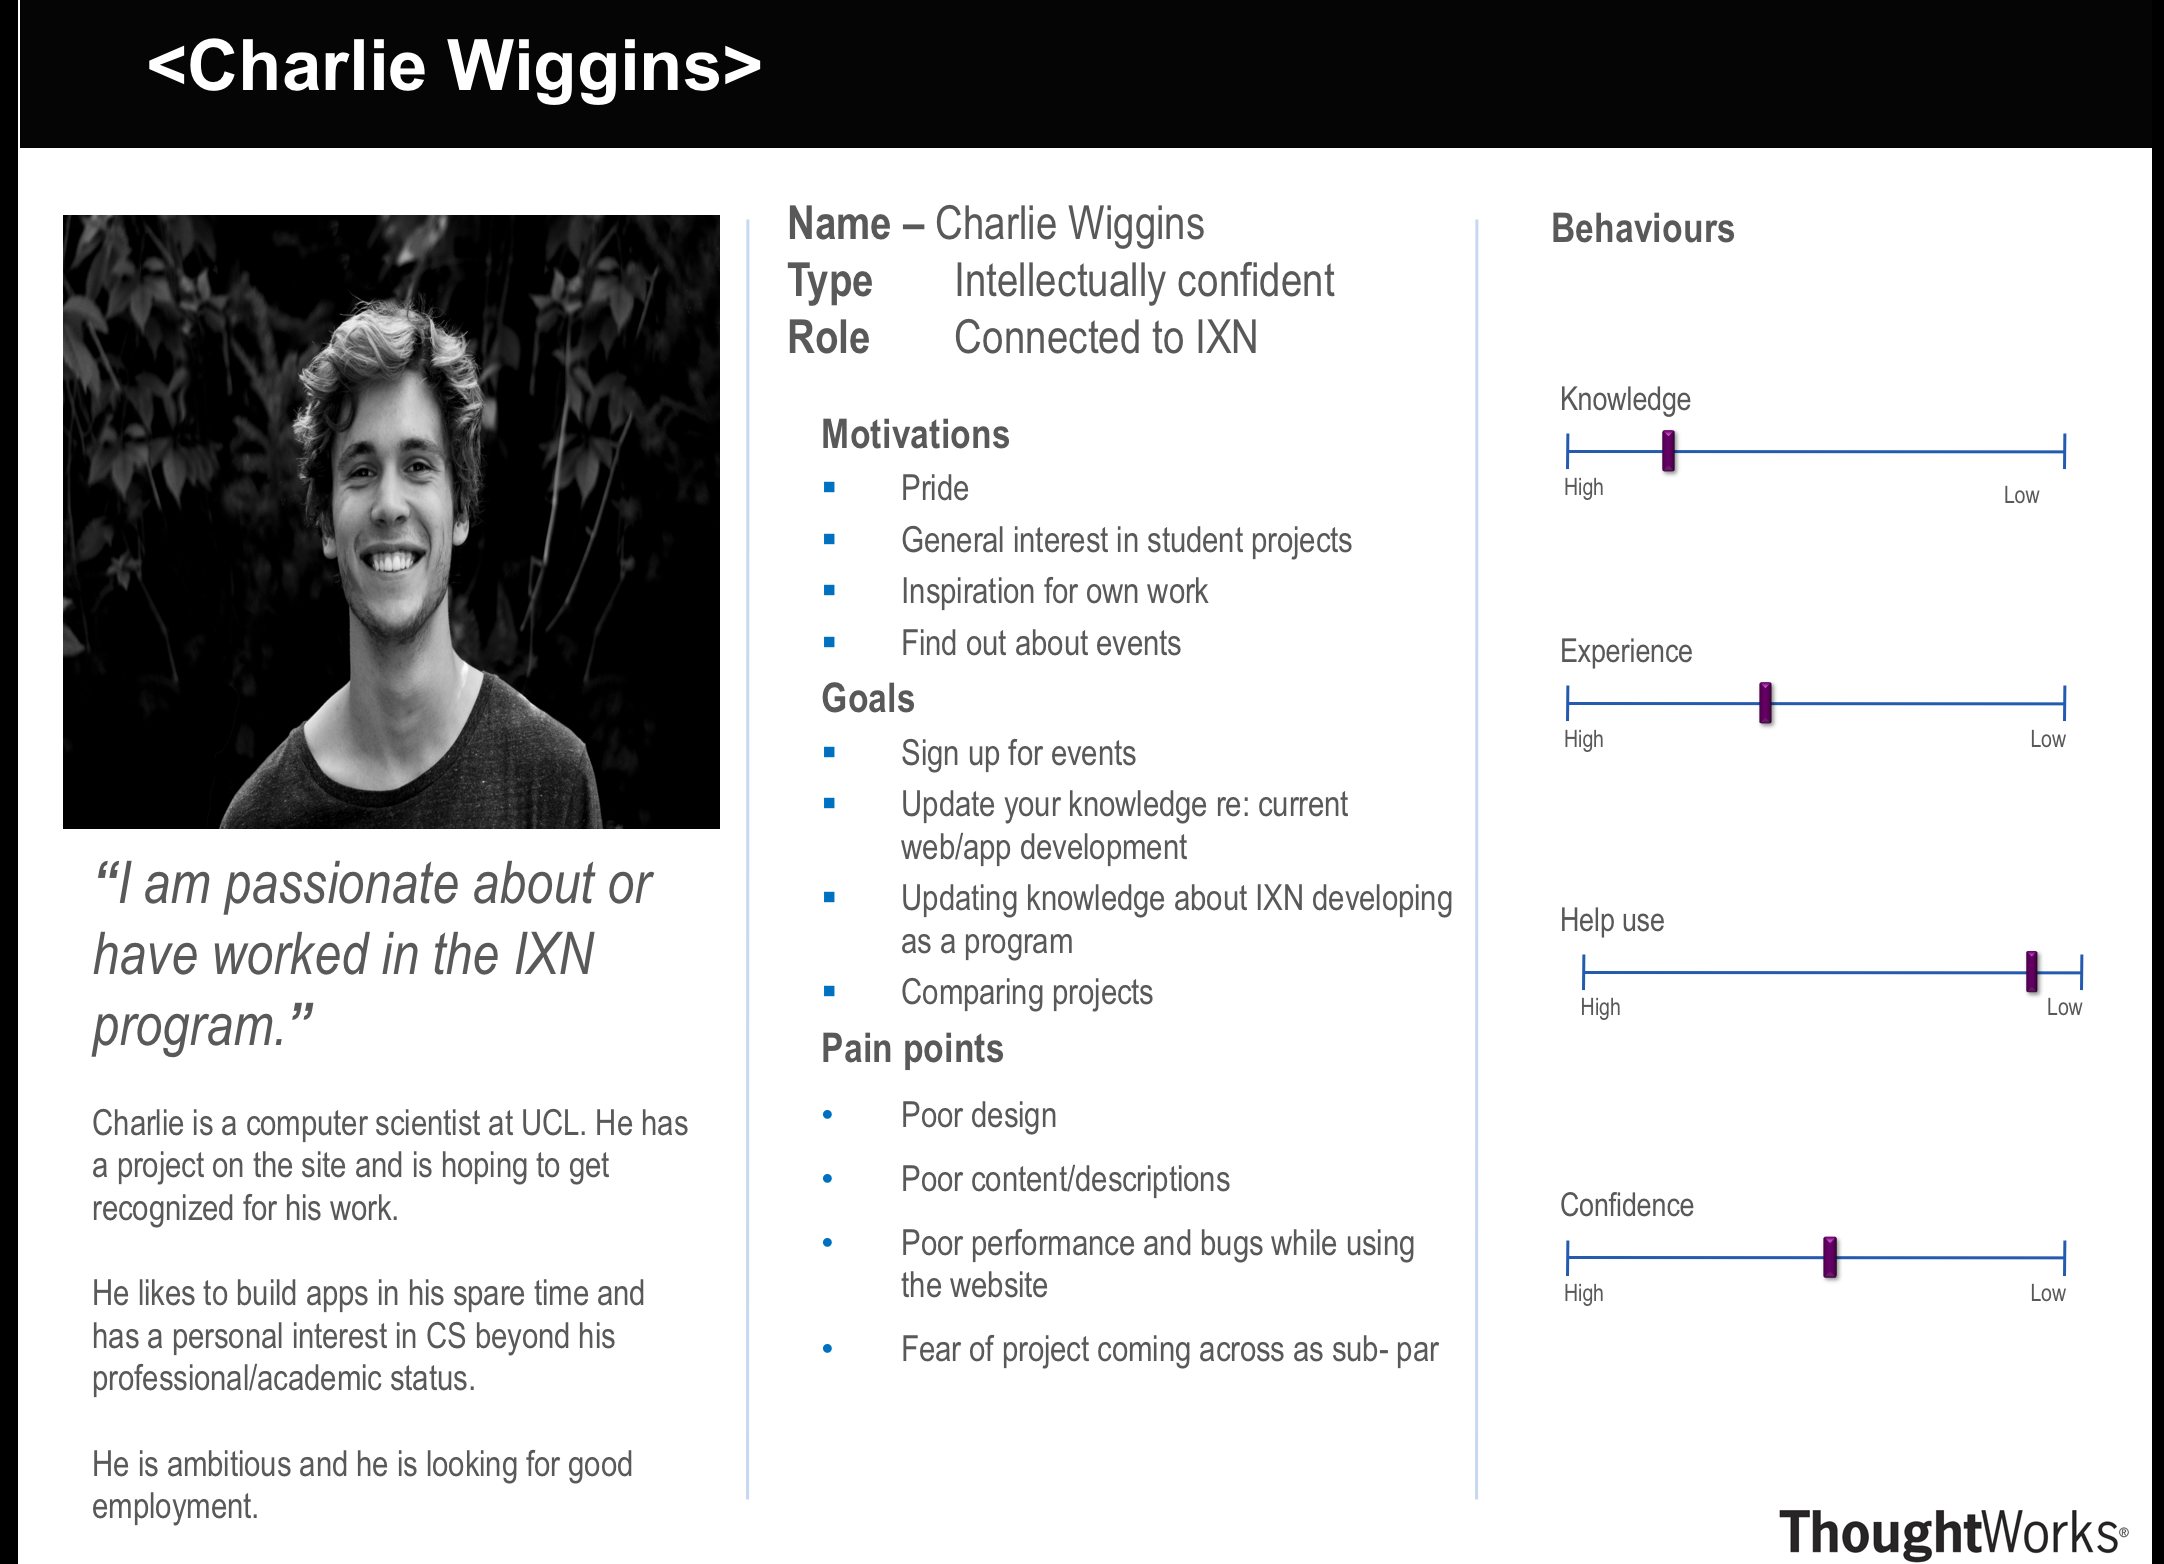
\includegraphics[trim = 0 0 0 0, clip, width=0.7\textwidth]{persona1.png}
      \caption{This is a persona}
      \label{persona1}
 \end{figure}

this image \cite{rumelt2012good} is of persona1 it is pretty good
\ref{persona1} \newpage

\hypertarget{technical-research}{%
\section{Technical Research}\label{technical-research}}

\newpage

\hypertarget{system-architecture}{%
\section{System Architecture}\label{system-architecture}}

In order to be able to create a high performance website, using the
latest technologies to optimises run time and speed up the design
process; a stack of Wordpress technologies were used in three tier
system architecture. The stack was run across both local and production
servers enabling a testing environment which was fully representative of
the production server while all code could be kept offline.

The full open source Roots stack \cite{rootsweb} was selected as it
provided all the tools and structure required to develop the project to
a professional standard. Figure \ref{systemarchitecture} shows the
relationship between the three roots technologies; Sage, Bedrock and
Trellis, and their relationship to the system architecture.

\begin{figure}[H]
\centering
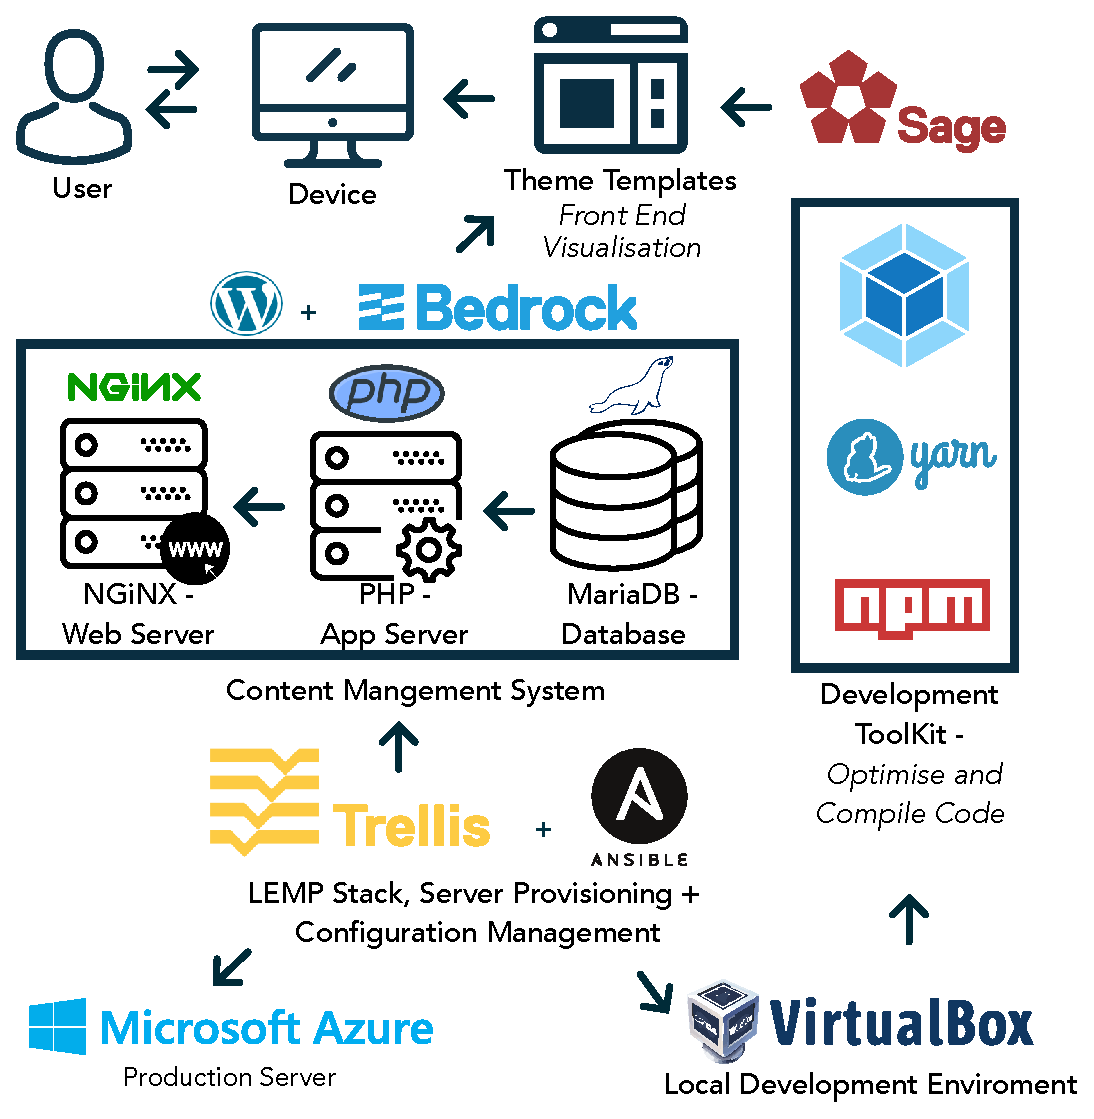
\includegraphics[trim = 0 0 0 0, clip, width=0.85\textwidth]{SystemArchitecture.eps}
\caption{Diagram showing the websites systems architecture, highlighting the relationship between different technologies}
\label{systemarchitecture}
\end{figure}

\newpage

\hypertarget{implementation}{%
\section{Implementation}\label{implementation}}

\hypertarget{testing}{%
\section{Testing}\label{testing}}

\newpage

\hypertarget{conclusion}{%
\section{Conclusion}\label{conclusion}}

\newpage
